\documentclass{standalone}
\usepackage{amsmath,amssymb,amsfonts} % Typical maths resource packages
\usepackage{tikz}
\usepackage{pgfplots}

\newcommand{\ry}{\pmb{y}}
\newcommand{\bP}[2]{\mathbb{P}_{#1} \left[ #2 \right]}
\begin{document}
    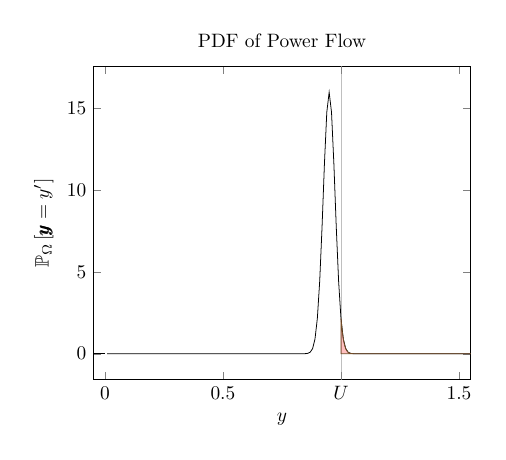
\begin{tikzpicture}[scale=.7]
      \begin{axis}[ title=PDF of Power Flow ,xlabel=$y$,ylabel=$\bP{\Omega}{\ry=y'}$, xmin=-.05, xmax=1.55, 
          xtick={0,.5,1.5},
  	  extra x ticks={1},
	  extra x tick style={grid=major},
	  extra x tick labels={$U$}
        ]
        \addplot+[black,no marks,domain=0.01:2,samples=200] { 1/(.025*sqrt(2*3.1415))*exp(-((x-.95)^2/(2*(.025^2))) };

        \addplot+[black,no marks, domain=-2:0,samples=5] {0};

        \addplot+[fill=red, fill opacity=.25,no marks,domain=1:2,samples=200] { 1/(.025*sqrt(2*3.1415))*exp(-((x-.95)^2/(2*(.025^2))) } \closedcycle;


        
      \end{axis}
    \end{tikzpicture}
\end{document}
